\documentclass[a4paper, 11pt]{article}

\usepackage[a4paper,margin=0.8in]{geometry}
\usepackage[english]{babel}
\usepackage[utf8]{inputenc}
\usepackage[T1]{fontenc}
\usepackage{lmodern}
\usepackage{listings}
\usepackage{graphicx}
\usepackage{amsmath}
\usepackage{framed}
\usepackage{amsfonts}
\usepackage{caption}
\usepackage{subcaption}
\usepackage{listings}
\usepackage{tabularx}
\usepackage{color}
\usepackage[dvipsnames]{xcolor}
\usepackage{fancyhdr}
\usepackage{lastpage}
% \usepackage[round, sort]{natbib}
\usepackage{tikz}
\usepackage{newverbs}
\usepackage{fancyvrb}
\usepackage{url}
\usepackage{hyperref}
\usepackage{titlesec}
\usepackage{dirtytalk}

\bibliographystyle {abbrv}
\usetikzlibrary{decorations.pathreplacing, matrix}

% \titleformat*{\section}{\fontsize{16}{20}\selectfont}
\titlespacing*{\section}{0em}{0em}{0.5em}

\graphicspath{{../imgs/}}
\interlinepenalty=10000

\definecolor{morange}{RGB}{237,106,90}
\definecolor{mgreen}{RGB}{63,127,95}
\definecolor{mpurple}{RGB}{127,0,85}

\lstset{
  basicstyle=\small\ttfamily, % Global Code Style
  captionpos=b, % Position of the Caption (t for top, b for bottom)
  extendedchars=true, % Allows 256 instead of 128 ASCII characters
  tabsize=2, % number of spaces indented when discovering a tab
  columns=fixed, % make all characters equal width
  keepspaces=true, % does not ignore spaces to fit width, convert tabs to spaces
  showstringspaces=false, % lets spaces in strings appear as real spaces
  breaklines=true, % wrap lines if they don't fit
  frame=trbl, % draw a frame at the top, right, left and bottom of the listing
  frameround=tttt, % make the frame round at all four corners
  framesep=4pt, % quarter circle size of the round corners
  numbers=left, % show line numbers at the left
  numberstyle=\tiny\ttfamily, % style of the line numbers
  commentstyle=\color{mgreen}, % style of comments
  keywordstyle=\color{mpurple}, % style of keywords
  stringstyle=\color{morange}, % style of strings
}


\newverbcommand{\rverb}{\color{BrickRed}}{}
\newverbcommand{\gverb}{\color{ForestGreen}}{}

% TAILLE DES PAGES (A4 serré)

\setlength{\intextsep}{1em}
\setlength{\parindent}{0pt}
\setlength{\parskip}{0.2em}
% \setlength{\textwidth}{17cm}
% \setlength{\textheight}{24cm}
% \setlength{\oddsidemargin}{-.7cm}
% \setlength{\evensidemargin}{-.7cm}
% \setlength{\topmargin}{-.5in}


\pagestyle{fancy}
\renewcommand{\headrulewidth}{0pt}
\renewcommand{\footrulewidth}{0.6pt}% default is 0pt
\lhead{}
\rhead{}
\lfoot{Page \thepage\ of \pageref{LastPage}}
\rfoot{Rémi Lespinet}
\cfoot{}
\cfoot{}

\newcounter{cquestion}
\renewcommand{\thecquestion}{\arabic{cquestion}}
\newenvironment{question}
{\par \vspace{0.5em} \noindent \stepcounter{cquestion} \hspace{-1em}
 $\bullet$ \underline{Q\thecquestion :}}
{}

\newenvironment{note}
{\begin{framed} \textbf{Note : }}
{\end{framed}}


% Commandes de mise en page
\newcommand{\file}[1]{\lstinline{#1}}
\newcommand{\name}[1]{\emph{#1}}
\newcommand{\Fig}[1]{Fig \ref{#1} p. \pageref{#1}}
\newcommand{\Figure}[1]{Figure \ref{#1} p. \pageref{#1}}
\newcommand{\Tab}[1]{Tab \ref{#1} p. \pageref{#1}}
\newcommand{\Table}[1]{Table \ref{#1} p. \pageref{#1}}
% \newcommand{\itemi}[1]{\item[$\bullet$]{\textbf{#1}}}
\newcommand{\itemi}[1]{\item{\textbf{#1}}}
% Commandes color
\newcommand{\colgood}[1]{\textcolor{ForestGreen} {#1}}
\newcommand{\colbad}[1]{\textcolor{BrickRed} {#1}}


% Commandes de maths
\newcommand{\function}[3]{#1 : #2 \to #3}
\newcommand{\intn}[2]{\left\{ #1 \dots #2 \right\}}
\newcommand{\intr}[2]{\left[ #1 ; #2 \right]}
\newcommand{\intro}[2]{\left] #1 ; #2 \right[}
\newcommand{\dotp}[2]{\langle #1, #2 \rangle}
\newcommand{\logn}[1]{\ln\left( #1\right)}
%% \newcommand{\det}[1]{\left| #1 \right|}
\newcommand{\pd}[2]{\frac{\partial #1}{\partial #2}}
\newcommand{\norm}[1]{\|#1\|}
\newcommand{\set}[2]{\left\{ #1 \hspace{.5em} ; \hspace{.5em}#2 \right\}}
\newcommand{\tr}[1]{Tr\left( #1 \right)}
\newcommand{\pcond}[2]{p(#1 \hspace{-.2em}\mid\hspace{-.2em} #2)}
\newcommand{\picond}[2]{\pi(#1 \hspace{-.2em}\mid\hspace{-.2em} #2)}
\newcommand{\parampicond}[3]{\pi_{#1}(#2 \hspace{-.2em}\mid\hspace{-.2em} #3)}
\newcommand{\e}[1]{\mathop{\mathbb{E}}\left[#1\right]}
\newcommand{\gradwrt}[2]{\nabla_{#1}{#2}}


\newcommand{\iid}{i.i.d }
\newcommand{\wrt}{w.r.t }

% Commandes informatique
\newcommand{\pfun}[1]{{\textbf{\texttt{#1}}}}

\newcommand{\ipart}[1]{\vspace{0.5em}\textbf{#1}\vspace{0.5em}}

\pagenumbering{arabic}

\title{\textsc{Algorithms for speech and natural language processing (MVA 2017/2018) \\ \emph{Homework 3}}}
\author{Rémi Lespinet}
\date{}

\begin{document}

\maketitle
\vspace{-1em}
\thispagestyle{fancy}


\section{Full pipeline}

Here's a description of the whole processing pipeline. I have used the
NLTK library for tokenization as well as pos tagging, and I've
implemented the rest myself.

% I'll resume the operation chain applied
% on tweets in the next section. I mention in each step if I've used
% NLTK for this operation or not.

\begin{enumerate}
  % \setlength\itemsep{-0.2em}
\itemi{Loading the input as UTF-8}
\itemi{Unescape HTML characters}

  This replaces characters like \verb+Mario +\rverb+&amp;+ \verb+Luigi+
  to \verb+Mario +\gverb+&+ \verb+Luigi+

\itemi{Multi-line reconstruction (Dynamic programming)}

  Because tweet are separated by newline characters but tweets can
  contain such character, there an ambiguity. I use a dynamic
  programming approach that tries to minimize an energy to find the
  best tweet separation (detailed in appendix
  \ref{sec:multi-line-tweets})

\itemi{Remove last words if the tweet is cut}

  Often in the corpus, tweets are cut because they are too long. When this happens, I
  remove the last letters up to the point where i find a space character.

\itemi{Remove emojis, links and @names (regex)}
\itemi{Process hashtags}

  Because sometimes the hashtags have a meaning, as in

  \verb+@HeralddeParis: City of+ \rverb+#Paris+ \verb+turns off the lights at the Eiffel Tower+

  If the hashtag word contains only characters and does not contain a
  case change, I keep it. This is a heuristic that works in the majority of cases

\itemi{Clean non ascii characters}
\itemi{Lower case everything}

  For the rest of the processing, I lower case all the text,
  % One again this is a heuristic that removes the case if there's no
  % change in case in the word.
  This changes

  \Verb[commandchars=\\\{\}]+So \colbad{DON'T BLAME THIS ON ALL}+
  $\to$
  \Verb[commandchars=\\\{\}]+So \colgood{don't blame this on all}+

  % By doing so we loseHere we lose information which is not

\itemi{Apply normalization and abbreviation dictionary}

  I use a
  \href{http://www.hlt.utdallas.edu/~yangl/data/Text_Norm_Data_Release_Fei_Liu}{normalization
    dictionary} and an abbreviation dictionary constructed from
  \href{http://www.smart-words.org/abbreviations/text.html}{this
    website}. This takes care of the one to many dependency and
  correct mistakes such as

  \begin{tabular}{lcl}
    \Verb[commandchars=\\\{\}]+... plans of going to Paris \colbad{omg}+
    & $\to$
    & \Verb[commandchars=\\\{\}]+... plans of going to Paris \colgood{oh my god}+
    \\
    \Verb[commandchars=\\\{\}]+I \colbad{dont} know why people ...+
    & $\to$
    & \Verb[commandchars=\\\{\}]+I \colgood{don't} know why people ...+
  \end{tabular}

  % \Verb[commandchars=\\\{\}]+... plans of going to Paris \colbad{omg}+
  % $\to$
  % \Verb[commandchars=\\\{\}]+... plans of going to Paris \colgood{oh my god}+




\itemi{Process english contractions}

  I use regex to transform constractions such as

  \Verb[commandchars=\\\{\}]+... to honor those \colbad{that've} been lost+
  $\to$
  \Verb[commandchars=\\\{\}]+... to honor those \colgood{that have} been lost+

  I do not process $'s$ as it can mean different things and it would
  require the context.

\itemi{Generate tokenization and post tagging (use NLTK Library)}

\itemi{Load contex2vec pretrained on ukwac}
\itemi{Cleanup the list of word used using NLTK dictionary}
\itemi{For each word in each tweet that is not a proper name}
  \begin{itemize}
  \item Run context2vec on this word, we obtain a context affinity vector $c$ of size
    $160000$ (size of the dictionary).
  \item Compute a list of candidate at edit distance less than 2 in
    the contex2vec dictionary using a precomputed tree structure (see
    appendix \ref{sec:fast-lookup-tree-structure})
  \item For each candidate $w$, compute the Damerau-Levensthein
    distance $d_w$. The formal similarity s is computed as
    $s_w = f(d)$. I've implemented the Damerau-Levenshtein version
    where each substring is updated at most one because I think that
    in our case, the full version slows down the computation and
    doesn't really improve.

  \item Calculate the likelihood using the context and the formal
    similarity as $l_w = s_w \cdot c_w$ for each candidate $w$
  \item Take the candidate word with maximum $l_w$ , if it's
    likelihood is below a threshold, keep the original word,
    otherwise use it instead.
  \end{itemize}
\end{enumerate}


\section{Successful examples}

Here's are some successful tweet outputs

\Verb[commandchars=\\\{\}]+I : \colbad{Tbh I'm} jealous my neighbor went to Paris with his \colbad{gf}!+ \\
\Verb[commandchars=\\\{\}]+O : \colgood{to be honest i am} jealous my neighbor went to Paris with his \colbad{girlfriend} !+

\Verb[commandchars=\\\{\}]+I : \colbad{@RT_com: #Paris txi} drivers turned off their meters, took people home for+\\
\Verb[commandchars=\\\{\}]+    free - reports \colbad{https://t.co/UUjfMTCXsM https://t.co/1TicKMbNJy}+ \\
\Verb[commandchars=\\\{\}]+O : \colgood{paris taxi} drivers turned off their meters , took people home for free - reports+

Here's an example that I've constructed (note that the were is corrected to where):

\Verb[commandchars=\\\{\}]+I : \colbad{idk} \colbad{were} \colbad{it'll} be next week, i \colbad{havent checkd atm}+ \\
\Verb[commandchars=\\\{\}]+O : \colgood{i do not know} \colgood{where} \colgood{it will} be next week, i \colgood{have not checked at the moment}+

% \Verb[commandchars=\\\{\}]+I : \colbad{omg} ! do \colbad{u kno were} i \colbad{cld fnid} it ?+\\
% \Verb[commandchars=\\\{\}]+O : \colgood{oh my god} ! do \colgood{you know where} i \colgood{could find} it ?+

\section{Failing examples}

\begin{enumerate}
\itemi{Parsing hashtags}

  The heuristic that I've introduced fail, which causes things such as

\Verb[commandchars=\\\{\}]+I : \colbad{@MalikRiaz:} My name is Malik Riaz. I am a Muslim. I condemn the \colbad{#ParisAttack}.+ \\
\Verb[commandchars=\\\{\}]+O : my name is malik riaz . i am a muslim . i condemn the .+

To solve the hashtag better we should try to decompose the hashtag into
different words and use the context to see if it is to be removed or not.

\itemi{Bigger abbreviation dictionary}

The dictionary of abbreviation is probably too small, we should use a
bigger one, for example the tweet

\Verb[commandchars=\\\{\}]+I : \colbad{@RajaOmarFarooq:} Prophet Muhammad \colbad{pbuh} only taught us Peace, Love and Respect+ \\
\Verb[commandchars=\\\{\}]+O : prophet muhammad \colbad{pbuh} only taught us peace , love and respect+

\itemi{Parsing date and time}

There's a lot of date and time in tweet, and the system currently does
not handle this.

\itemi{Pronunciation related mistakes}

There are also pronunciation related mistakes such as homophones which
are not correctly handled when the words have different spelling such as

\Verb[commandchars=\\\{\}]+I : Turn left, then \colbad{write} and you'll find it !+ \\
\Verb[commandchars=\\\{\}]+O : turn left , then \colbad{write} and you will find it !+

We could use a homophone dictionary here and use contex2vec
independently of the edit distance.

\itemi{Too many mistakes in the input}


When there is too much mistakes, this becomes really hard because
context2vec doesn't know the majority of the word in the context, which is
why normalization and abbreviation dictionaries are very important.
For example with the sentence in the previous example

\Verb[commandchars=\\\{\}]+I : do \colbad{u kno were} i \colbad{cld fnid} it ?+

the system succeed to find the correct sentence :

\Verb[commandchars=\\\{\}]+O : do \colgood{you know where} i \colgood{could find} it ?+

This is possible because \emph{u} and \emph{cld} are in the
dictionary, if I replace \emph{cld} by \emph{cuold} we obtain

\Verb[commandchars=\\\{\}]+I : do \colbad{u kno were} i \colbad{cuold fnid} it ?+ \\
\Verb[commandchars=\\\{\}]+O : \colgood{do you know where} i \colbad{cuold fnid} it ?+




% \Verb[commandchars=\\\{\}]+I : The #EmpireStateBuilding went dark at 10:00 PM/ET on Friday, November 13, 2015+
% \Verb[commandchars=\\\{\}]+I : the went dark at 10:00 pm/et on friday , november 13 , 2015+

\end{enumerate}



% There are also pronunciation related mistakes such as homophones which
% are not correctly handled when the words have different spelling such as

% \Verb[commandchars=\\\{\}]+I : Turn left, then \colbad{write} and you'll find it !+ \\
% \Verb[commandchars=\\\{\}]+O : turn left , then \colbad{write} and you will find it !+



% This was very interesting to design our own, but it was hard to do in
% one week,

\section{Conclusion}

There's a huge room for improvement, tweets are really hard to
normalize. They can really contain anything : some use different
languages, the hashtags sometimes play both the role of a word, emojis
or smileys can also be used as words, etc...

In the end, I was very surprised about the quality that we can obtain
with this \say{simple} model. I think we can get better
results by training context2vec on a clean corpus of tweets.

\appendix
\newpage
\section{Multi-line tweets}
\label{sec:multi-line-tweets}

In the input corpus, each tweet is separated with a newline character,
but tweets can also contain such characters, which makes the task of
reconstructing tweets ambiguous. Even though this is not the main
point of the homework, I've implemented a heuristic algorithm that
does this processing. It is based on the following observations
\begin{itemize}
\item Tweets in the corpus cannot be longer than 140 characters
\item The string \verb+RT+ in a newline almost surely marks the end of
  a character
\item The unicode character \verb+...+ marks the end of a tweet (that
  has been cut because too long)
\end{itemize}
The algorithm tries to find tweet delimitations by minimizing an
energy by dynamic programming
% \begin{displaymath}
%   \min_\sigma \sum_{i=1}^n S(w_{\sigma(i)}, \dots w_{\sigma_{(i+1)}})
% \end{displaymath}
% where $n$ is the minimum number of tweets that fit the input and
\begin{displaymath}
  S(w_i, \dots w_j) = \left\{
    \begin{array}{ll}
      \left(\dfrac{1}{K}\text{len}(w_1, \dots w_n) - \sum_{k = i}^j \text{len}(w_i)\right)^2 & \text{ if } \sum_{k = i}^j \text{len}(w_i) < 140 \\
      \min_{i \le k \le j} S(w_i, w_k) + S(w_{k+1}, w_j) & \text{ otherwise }
    \end{array}
  \right.
\end{displaymath}
Where $K$ is the minimum number of tweets that fit the input.

\newpage
\section{Fast lookup tree structure}
\label{sec:fast-lookup-tree-structure}

If we want to correct each word based on the formal similarity and
context similarity, we want to compute, for each word $w$ of the
sentence the edit distance with the contex2vec dictionary. This is
very costly as it requires to process all the dictionary at each step.
To solve this problem, I noticed that a word $s$ can not be at edit
distance less than $2$ to a word $t$ if $t$ contains 2 or more character
that $s$ doesn't have.

To exploit this, I encode each word of the contex2vec dictionary
as a bag of letter, which gives me a vector (whose size is the number
of elements in the alphabet $\mathcal{A}$)

I look at the letter $\hat{\alpha}$ that differentiate the most the
words (given a letter $\alpha \in \mathcal{A}$, I separate the
dictionary in two sets, the words that have this letter $X_\alpha$,
and the words that doesn't $\bar{X}_\alpha$, and I compute
\begin{displaymath}
  \hat{\alpha} = \arg\min_{\alpha \in \mathcal{A}} | {X_\alpha - \bar{X}_\alpha} |
\end{displaymath}
I can then apply the same operation recursively on the subdictionaries
$X_{\hat{\alpha}}$ and $\bar{X}_{\hat{\alpha}}$ with the modified alphabet
$\mathcal{A} - \{\hat{\alpha}\}$.  By doing so I construct a tree that
can be used to get candidate words in the dictionary very fast by
crawling the tree. A simplified view of the crawling part is given below

\begin{lstlisting}[language=Python]
def CRAWL_TREE(T, word, edit=2):

    if edit < 0 or T is a leaf:
        return T.data

    if T.letter in word:
        left  = CRAWL_TREE(T.left, word, edit-1)
        right = CRAWL_TREE(T.right, word, edit)
    else:
        left  = CRAWL_TREE(T.left, word, edit)
        right = CRAWL_TREE(T.right, word, edit-1)

    return concatenate(left, right)
\end{lstlisting}

Using this structure it is guaranteed to retrieve the words at edit
distance 2 or less, but of course the list returned also contains
words at edit distance more than 2 in the general case.
We could improve this structure by considering repetition of letters
and splitting better the dictionary (right now the algorithm is greedy),
but in practice the number of words retrieved is in the order of $10^2$ while
the number of words in the dictionary is in the order of $10^5$


\end{document}

%% \begin{figure}[p]
%%   \centering
%%   \begin{subfigure}[t]{0.40\textwidth}
%%     \centering
%%     \includegraphics[width=\textwidth]{LDA_classificationA_train}
%%     \caption{Training observations A ($150$ points)}\label{fig:LDA-A-train}
%%   \end{subfigure}
%%   \quad
%%   \begin{subfigure}[t]{0.40\textwidth}
%%     \centering
%%     \includegraphics[width=\textwidth]{LDA_classificationA_test}
%%     \caption{Test observations A ($1500$ points)}\label{fig:LDA-A-test}
%%   \end{subfigure}
%%   \vskip\baselineskip
%%   \begin{subfigure}[t]{0.40\textwidth}
%%     \centering
%%     \includegraphics[width=\textwidth]{LDA_classificationB_train}
%%     \caption{Training observations B ($150$ points)}\label{fig:LDA-B-train}
%%   \end{subfigure}
%%   \quad
%%   \begin{subfigure}[t]{0.40\textwidth}
%%     \centering
%%     \includegraphics[width=\textwidth]{LDA_classificationB_test}
%%     \caption{Test observations B ($1500$ points)}\label{fig:LDA-B-test}
%%   \end{subfigure}
%%   \vskip\baselineskip
%%   \begin{subfigure}[t]{0.40\textwidth}
%%     \centering
%%     \includegraphics[width=\textwidth]{LDA_classificationC_train}
%%     \caption{Training observations C ($150$ points)}\label{fig:LDA-C-train}
%%   \end{subfigure}
%%   \quad
%%   \begin{subfigure}[t]{0.40\textwidth}
%%     \centering
%%     \includegraphics[width=\textwidth]{LDA_classificationC_test}
%%     \caption{Test observations C ($1500$ points)}\label{fig:LDA-C-test}
%%   \end{subfigure}
%%   \caption{Sample data and decision boundary representation for the LDA classifier on the three files}\label{fig:LDA}
%% \end{figure}




  % \begin{table}[h!]
  %   \centering
  %   \begin{tabular}{|c|c|c|c||c|c|c|}
  %     \hline
  %     & \multicolumn{3}{c||}{\textbf{a0}} & \multicolumn{3}{c|}{\textbf{a1}}\\
  %     \hline
  %     & s0 & s1 & s2 & s0 & s1 & s2 \\
  %     \hline
  %     s0 & 0.45 & 0.00 & 0.55 & 0.00 & 0.00 & 1.00 \\
  %     s1 & 0.00 & 0.00 & 1.00 & 0.50 & 0.40 & 0.10 \\
  %     s2 & 0.60 & 0.00 & 0.40 & 0.00 & 0.90 & 0.10 \\
  %     \hline
  %   \end{tabular}
  %   \captionof{table}{Representation of the transition table
  %     corresponding to the graph} \label{tab:transition-table}
  % \end{table}

  % \begin{figure}[h]
  %   \centering
  %   \includegraphics[width=0.7\textwidth]{VI_convergence}
  %   \caption{Convergence of the value iteration algorithm}\label{fig:VI-convergence}
  % \end{figure}


  % \begin{figure}[ht]
  %   \centering
  %   \begin{subfigure}[t]{0.48\textwidth}
  %     \centering
  %     \includegraphics[width=\textwidth]{ex1_bernoulli_arms_2}
  %     \caption{Representations of the parameters of each arms}\label{fig:ex1-bernoulli-arms-2}
  %   \end{subfigure}
  %   \quad
  %   \begin{subfigure}[t]{0.48\textwidth}
  %     \centering
  %     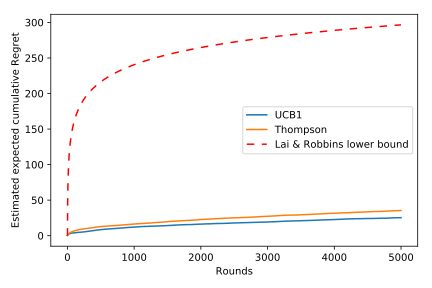
\includegraphics[width=\textwidth]{ex1_bernoulli_regret_2}
  %     \caption{Estimated expected cumulative regret for UCB1 and TS,
  %       and Lai-Robbins lower bound}\label{fig:ex1-bernoulli-arms-regret-2}
  %   \end{subfigure}
  %   \caption{Representation of the arms means and expected cumulative
  %     regret for the second chosen Bernoulli bandit}\label{fig:ex1-bernoulli-2}
  % \end{figure}
